\documentclass[11pt, a4paper]{article}
\input{preamble.tex}
\switchlang{ru}
\begin{document}

\title{1989 "--- Aero trackball}
\date{}
\maketitle
\selectlanguage{russian}
Aero trackball, показанный на рисунке \ref{fig:AeroPhoto}, был выпущен на рынок тайваньской компанией ICA Technology в 1990 году \cite{mouses4, mouses5}. Рекламные материалы \cite{mouses5} упоминают использованные в трекболе <<продвинутые опто-механические технологии, динамическое разрешение: от 100 до 1000 dpi, обычно установленное в 200 dpi>> (то есть, очевидно, имеет место программное масштабирование разрешающей способности), а также <<улучшенные электронные часы>>, являющиеся частью трекбола.

\begin{figure}[h]
    \centering
    
\includegraphics[scale=0.6]{1990_aero_trackball/pic_30.jpg}
    \caption{Изображение Aero trackball}
    \label{fig:AeroPhoto}
\end{figure}

Корпус трекбола выполнен в футуристической манере 80-х годов с соответствующими этому стилю прямоугольными формами и изломанными гранями. Основная часть выполнена из бежевого пластика. На верхней части корпуса расположены три большие серые кнопки. Клавиши трекбола, которые показаны на рисунке \ref{fig:AeroTopBottom} как нижняя левая и нижняя правая, соответствуют левой и средней клавишам мыши, а роль правой клавиши играет верхняя правая клавиша трекбола. Шар диаметром около 4,5 см размещён в центре корпуса. Наконец, в верхней левой части корпуса расположены цифровые часы.

На нижней стороне можно увидеть ребристую муфту, защищающую кабель от повреждения в месте выхода из корпуса, ярлык с техническими данными, резиновые ножки, обеспечивающие устойчивое положение устройства на поверхности стола, а также переключатель, позволяющий выбрать режим информационного обмена с компьютером.

Очевидно, по замыслу разработчиков размеры и форма трекбола должны гармонировать с размером и формой современных ему клавиатур. Из-за этого, а также с учетом не самого крупного шара, устройство получилось плоским, но весьма габаритным (рис. \ref{fig:AeroSize}).

\begin{figure}[h]
    \centering
    
\includegraphics[scale=0.68]{1990_aero_trackball/top_30.jpg}
    
\includegraphics[scale=0.68]{1990_aero_trackball/bottom_30.jpg}
    \caption{Aero trackball, вид сверху и снизу}
    \label{fig:AeroTopBottom}
\end{figure}

ICA Technology разработала трекбол Aero с учетом особенностей строения кисти человека, и несмотря на футуристические изломанные формы, положение руки на корпусе оказывается достаточно удобным (рис. \ref{fig:AeroHand}), а кнопки большого размера также добавляют ему удобства использования. Очевидным недостатком трекбола является невозможность извлечь шар для чистки без разбора корпуса.

\begin{figure}[h]
    \centering
    
\includegraphics[scale=0.39]{1990_aero_trackball/size.jpg}
    \caption{Изображение Aero trackball на размерном коврике с шагом сетки 1~см}
    \label{fig:AeroSize}
\end{figure}

В зависимости от положения переключателя, трекбол совместим протоколом двухкнопочной мыши Microosft (<<MS>>) и трехкнопочной мыши Mouse Systems (<<PC>>). В комплект поставки входит драйвер с программами установки и тестирования, программа для создания и вызова пользовательского меню, что позволяет использовать Aero Trackball для ввода управляющих команд в популярных приложениях, не поддерживающих работу с мышью. В пакет также входит графический редактор для DOS.

\begin{figure}[h]
    \centering
    
\includegraphics[scale=0.38]{1990_aero_trackball/hand_30.jpg}
    \caption{Изображение Aero trackball с моделью руки человека}
    \label{fig:AeroHand}
\end{figure}

Трекбол в разобранном виде показан на рисунке \ref{fig:AeroInside}. Как можно видеть, технически это достаточно стандартная по меркам 90-х годов оптомеханическая конструкция, а также блок электронных часов, для удобства сборки дополнительно прикрепленных к верхней части корпуса с помощью бумажной липкой ленты и не подсоединенных ни к компьютеру, ни к блоку электроники трекбола.

\begin{figure}[h!]
    \centering
    
\includegraphics[scale=0.53]{1990_aero_trackball/inside_30.jpg}
    \caption{Изображение Aero trackball в разобранном виде}
    \label{fig:AeroInside}
\end{figure}



В обзоре, представленном в \cite{mouses4}, деликатно отмечается, что часы, встроенные в трекбол, имеют собственный источник питания и поэтому не зависят от компьютера. Таким образом, жидкокристаллический дисплей в составе устройства не несет никаких других функций кроме отображения текущего времени и не управляется программно. Также, учитывая невозможность извлечения часов без разборки устройства, замена их источника питания (роль которого играет обычная для малогабаритных часов батарейка) явно не рассматривалась как приоритетная задача при разработке трекбола.

Извлечение часов из корпуса показывает, что они по всей видимости были изначально предназначены для продажи в качестве самостоятельного изделия. Во всяком случае, их корпус снабжён откидной подставкой для установки на поверхности стола (рис. \ref{fig:AeroClock}). Регулировка отображаемого времени осуществляется способом, стандартным для электронных часов 1970-х годов, с помощью двух кнопок на их передней панели.

\begin{figure}[h]
    \centering
    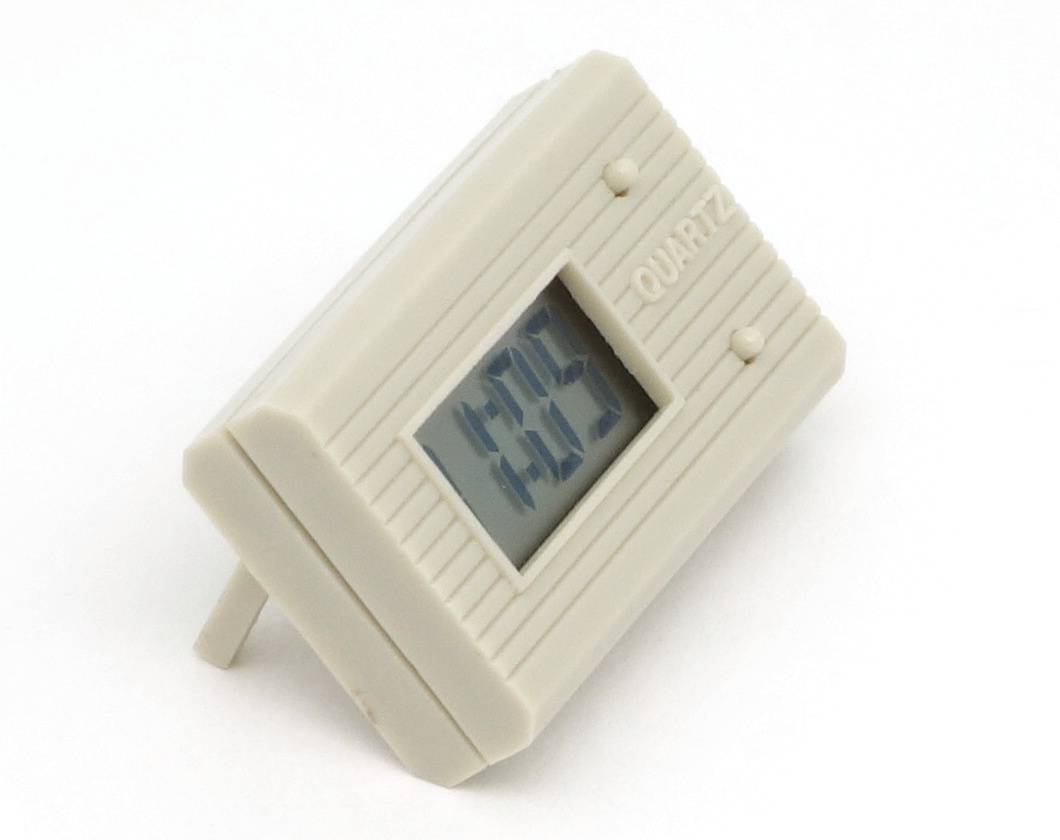
\includegraphics[scale=0.8]{1990_aero_trackball/clock_30.jpg}
    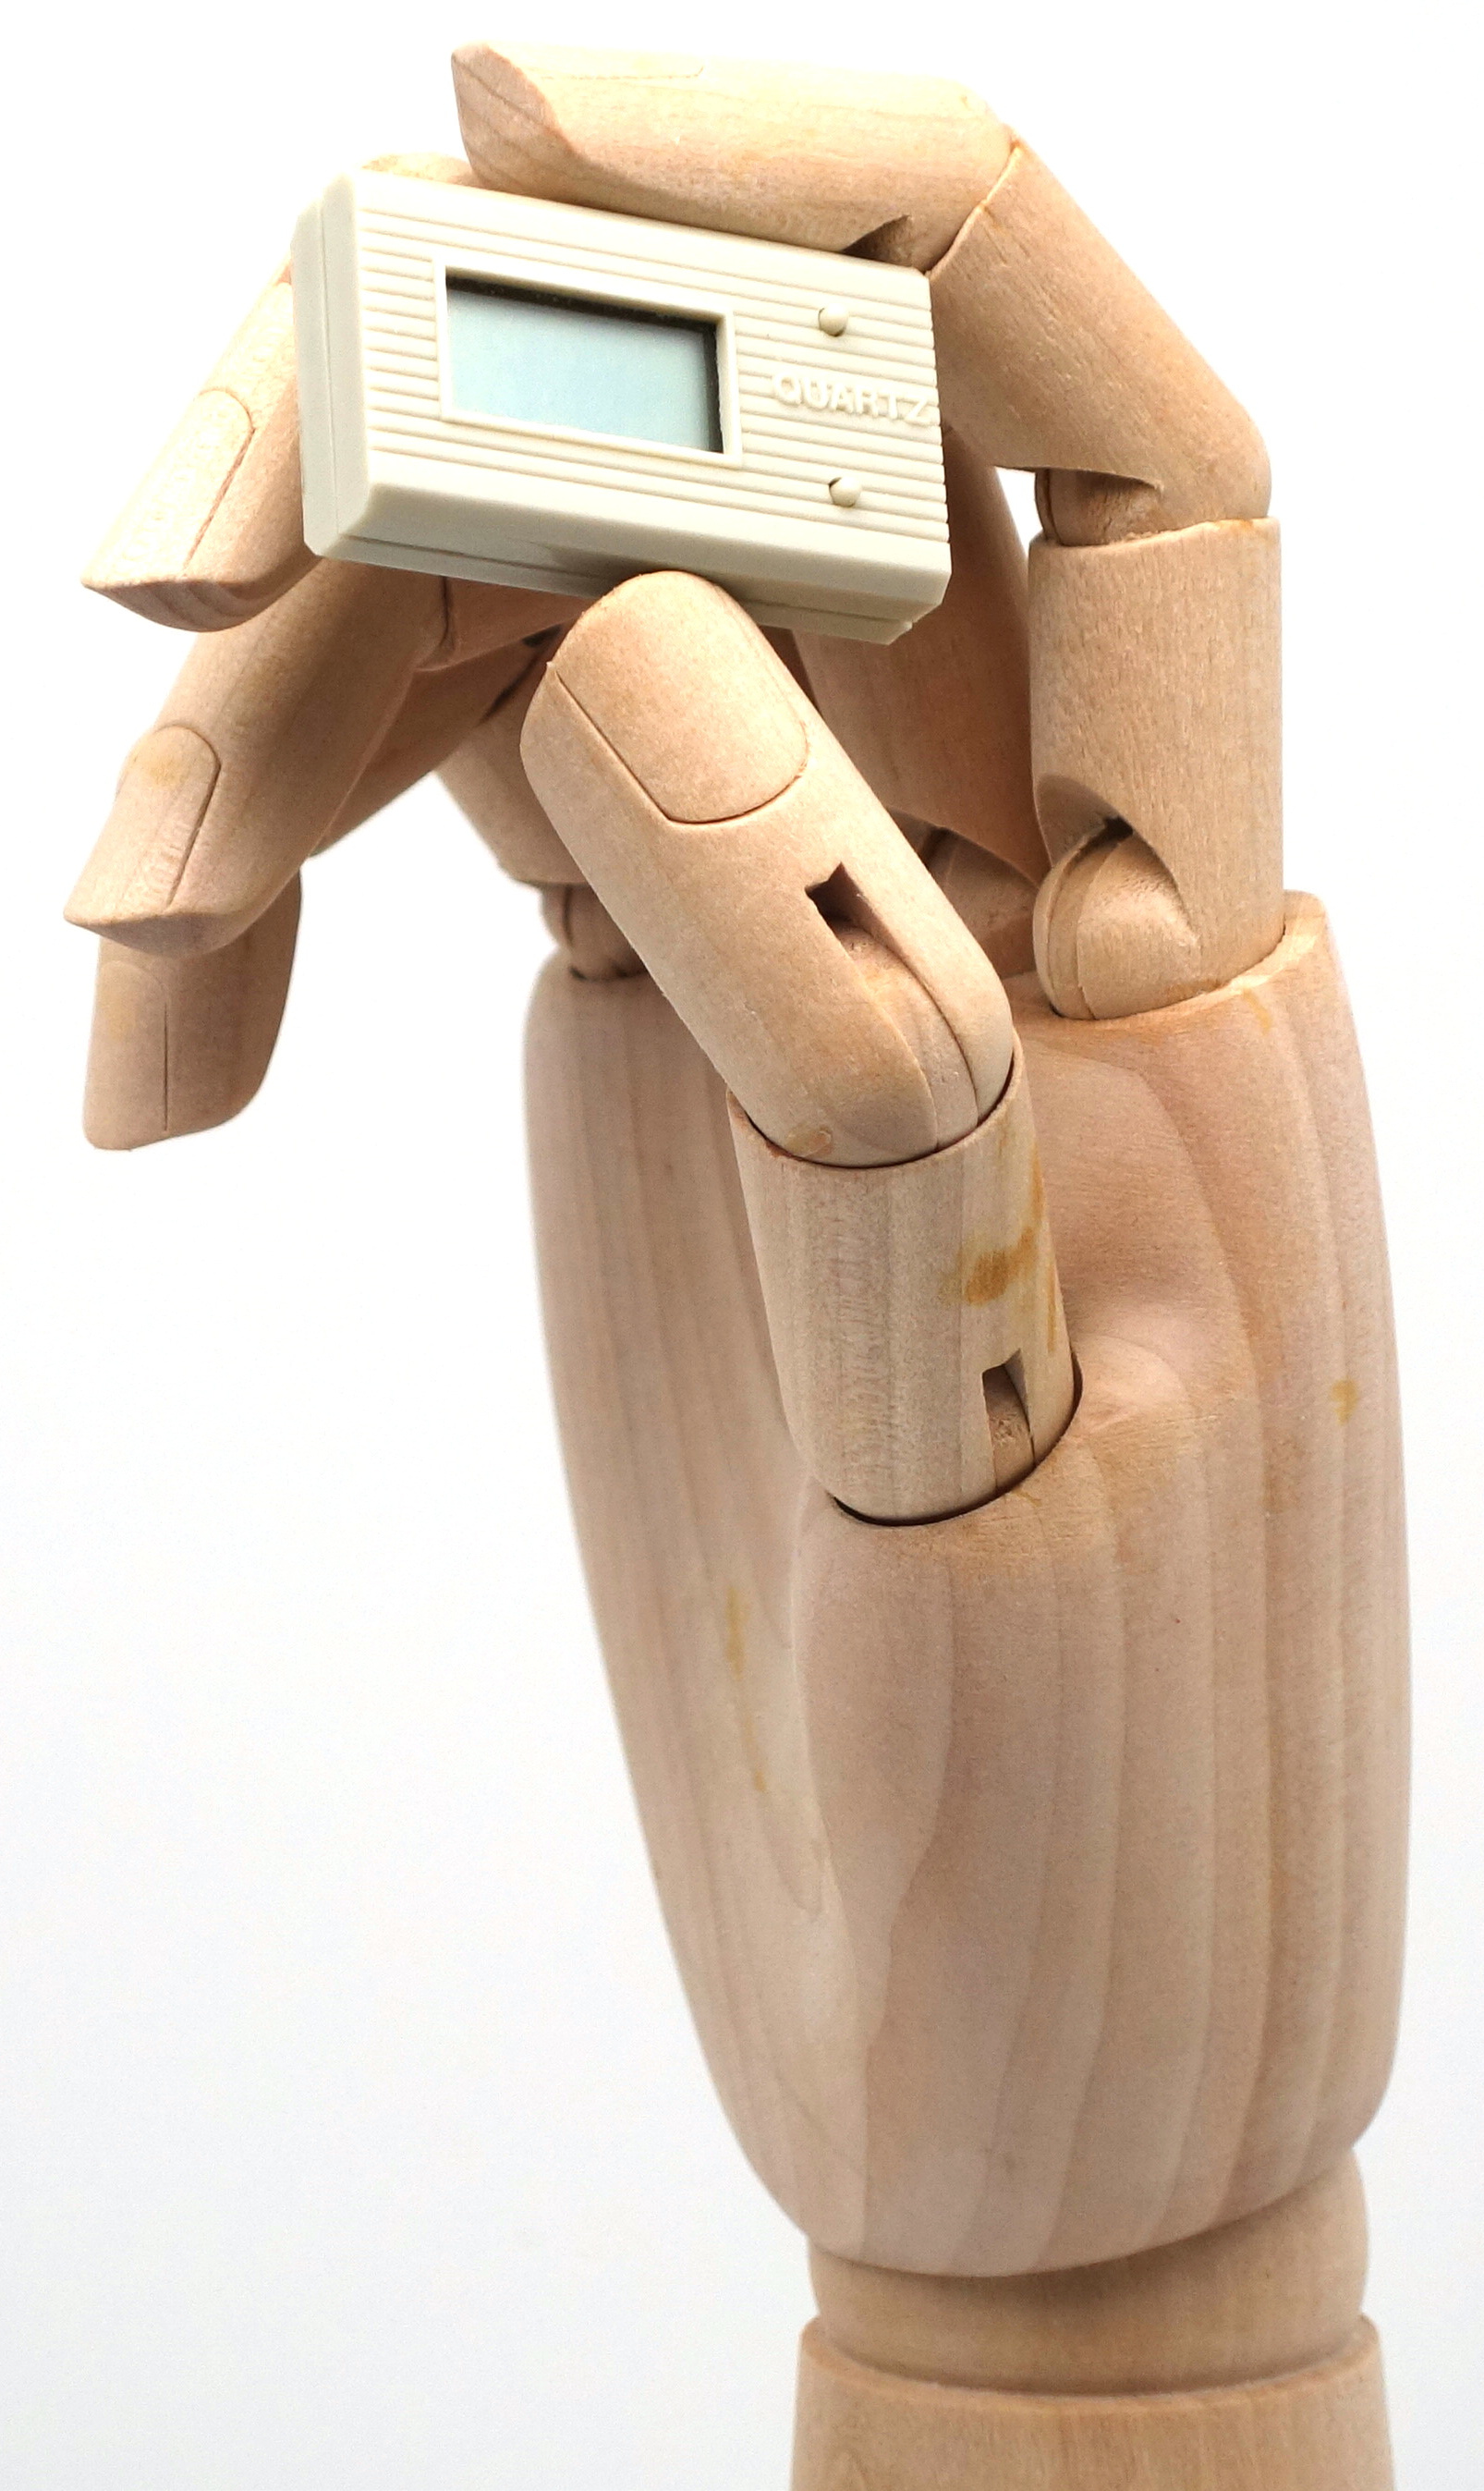
\includegraphics[scale=0.6]{1990_aero_trackball/hand_clock_30.jpg}
    \caption{Часы, извлеченные при разборке Aero trackball}
    \label{fig:AeroClock}
\end{figure}

\begin{thebibliography}{9}
	\bibitem {mouses4} Zmaga s cistim tusem // Moj Micro, No. 4, April 1991. P. 14--15. \url{https://archive.org/details/Moj_Micro_1991_04/page/n13/mode/2up}
	\bibitem {mouses5} Aero trackball reaches your fingers // BYTE, February 1991, P. 74. \url{https://archive.org/details/eu_BYTE-1991-02_OCR/page/n153/mode/2up}
\end{thebibliography}
\end{document} 
